\documentclass{article}
\usepackage{mathrsfs}
\usepackage{amsmath}
\usepackage{amsthm}
\usepackage{amssymb}
\usepackage{graphicx}
\usepackage{color}
%\include{macros}
%\usepackage{floatflt}
%\usepackage{graphics}
%\usepackage{epsfig}
\usepackage{float}%稳定图片位置
\usepackage{graphicx}%画图
\newcommand{\reals}{{\mathbb{R}}}
\newcommand{\dom}{{\bf{dom}}}
\newcommand{\symm}{{\bf{S}}}
\newcommand{\Tr}{{\bf{tr}}}

\theoremstyle{definition}
\newtheorem{theorem}{Theorem}[section]
\newtheorem{lemma}[theorem]{Lemma}
\newtheorem{proposition}[theorem]{Proposition}
\newtheorem{corollary}[theorem]{Corollary}

\theoremstyle{definition}
\newtheorem*{defition}{Definition}
\newtheorem*{example}{Example}

\theoremstyle{remark}
\newtheorem*{remark}{Remark}
\newtheorem*{note}{Note}
\newtheorem*{exercise}{Exercise}

\setlength{\oddsidemargin}{-0.25 in}
\setlength{\evensidemargin}{-0.25 in} \setlength{\topmargin}{-0.25
in} \setlength{\textwidth}{7 in} \setlength{\textheight}{8.5 in}
\setlength{\headsep}{0.25 in} \setlength{\parindent}{0 in}
\setlength{\parskip}{0.1 in}

\newcommand{\homework}[4]{
\pagestyle{myheadings} \thispagestyle{plain}
\newpage
\setcounter{page}{1} \setcounter{section}{#4} \noindent
\begin{center}
\framebox{ \vbox{\vspace{2mm} \hbox to 6.28in { {\bf
VE485,~Optimization~in~Machine~Learning (Summer 2020) \hfill Homework: #1} }
\vspace{6mm} \hbox to 6.28in { {\Large \hfill #1 \hfill} }
\vspace{6mm} \hbox to 6.28in { {\it Lecturer: #2 \hfill} }
\vspace{2mm} \hbox to 6.28in { {\it Student: #3 \hfill} }
\vspace{2mm} } }
\end{center}
\markboth{#1}{#1} \vspace*{4mm} }


\begin{document}

\homework{2. Convex Function}{Xiaolin Huang \hspace{5mm} {\tt
xiaolinhuang@sjtu.edu.cn}}{Chongdan Pan
\hspace{5mm} {\tt panddddda@sjtu.edu.cn } }{9}

%%%%%%%%%%%%%%%%%%%%%%%%%%%%%%%%%%%%%%%%%%%%%%%%%%%%%%%%%%%%%%%%%%%%
% Section 2.  Problem
%%%%%%%%%%%%%%%%%%%%%%%%%%%%%%%%%%%%%%%%%%%%%%%%%%%%%%%%%%%%%%%%%%%%

\section*{Problem 1} \label{ex-midpoint-cvx}
\emph{Definition of convexity.}
Suppose  $ f: \reals \rightarrow \reals $  is convex, and  $a,~b \in \dom f $  with  $ a < b $ .

\begin{enumerate}
\item Show that
\[
f(x) \leqslant \frac{b-x}{b-a}f(a) + \frac{x-a}{b-a}f(b)
\]
for all  $ x \in [a,b] $ .

\item Show that
\[
\frac{f(x)-f(a)}{x-a} \leqslant \frac{f(b)-f(a)}{b-a}
\leqslant  \frac{f(b)-f(x)}{b-x}
\]
for all  $ x \in (a,b) $ .
Draw a sketch that illustrates this inequality.

\item Suppose  $ f $  is differentiable.  Use the result in 2 to show that
\[
f'(a) \leqslant \frac{f(b)-f(a)}{b-a} \leqslant f'(b).
\]
Note that these inequalities also follow from (3.2) in the textbook :
\[
f(b) \geqslant f(a) + f'(a)(b-a), \qquad
f(a) \geqslant f(b) + f'(b)(a-b).
\]

\item  Suppose  $ f $  is twice differentiable.
Use the result in 3 to show that  $ f''(a) \geqslant 0 $  and $ f''(b) \geqslant 0 $ .
\end{enumerate}


{\bf{Answer
    \\\\\begin{enumerate}
    \item (a)  Since $f(x)$ is convex, then $f(\theta a+(1-\theta)b)\leq\theta f(a)+(1-\theta)f(b), \forall \theta$
    \\Let $x=\theta a+(1-\theta)b$, then $\theta=\frac{b-x}{b-a},1-\theta=\frac{x-a}{b-a}$
    \\Then $f(x)\leq \frac{b-x}{b-a}f(a)+\frac{x-a}{b-a}f(b)$
    \item (b) $f(a)\geq f(x)+\nabla f(x)^\mathrm{T}(a-x)$
    \\$\nabla f(a)^\mathrm{T}\leq\frac{f(x)-f(a)}{x-a}\leq\nabla f(x)^\mathrm{T}$
    \\Similarly, $\nabla f(x)^\mathrm{T}\leq\frac{f(b)-f(x)}{b-x}\leq\nabla f(b)^\mathrm{T}$
    \\Then $\frac{f(x)-f(a)}{x-a}\leq\frac{f(b)-f(x)}{b-x}$
    \\\\$xf(a)+bf(x)-bf(a)\leq xf(b)+af(x)-af(b)$
    \\Plus $bf(b)$ on both sides, we get $bf(b)+xf(a)-bf(a)-xf(b)\leq bf(b)+af(x)-af(b)-bf(x)$
    \\$(b-x)(f(b)-f(a)\leq (b-a)(f(b)-f(x))$
    \\Then $\frac{f(b)-f(a)}{b-a}\leq\frac{f(b)-f(x)}{b-x}$
    \\\\Similarly, we can plus $af(a)$ on both sides, we get $af(a)+bf(x)-bf(a)-af(x)\leq af(a)+xf(b)-af(b)-xf(a)$
    \\$(a-b)(f(a)-f(x))\leq(a-x)(f(a)-f(b))$
    \\Then $\frac{f(x)-f(a)}{x-a}\leq\frac{f(b)-f(a)}{b-a}$  
    \\\\Therefore $\frac{f(x)-f(a)}{x-a}\leq\frac{f(b)-f(a)}{b-a}\leq\frac{f(b)-f(x)}{b-x}$ 
    \begin{figure}[H]
        \centering
        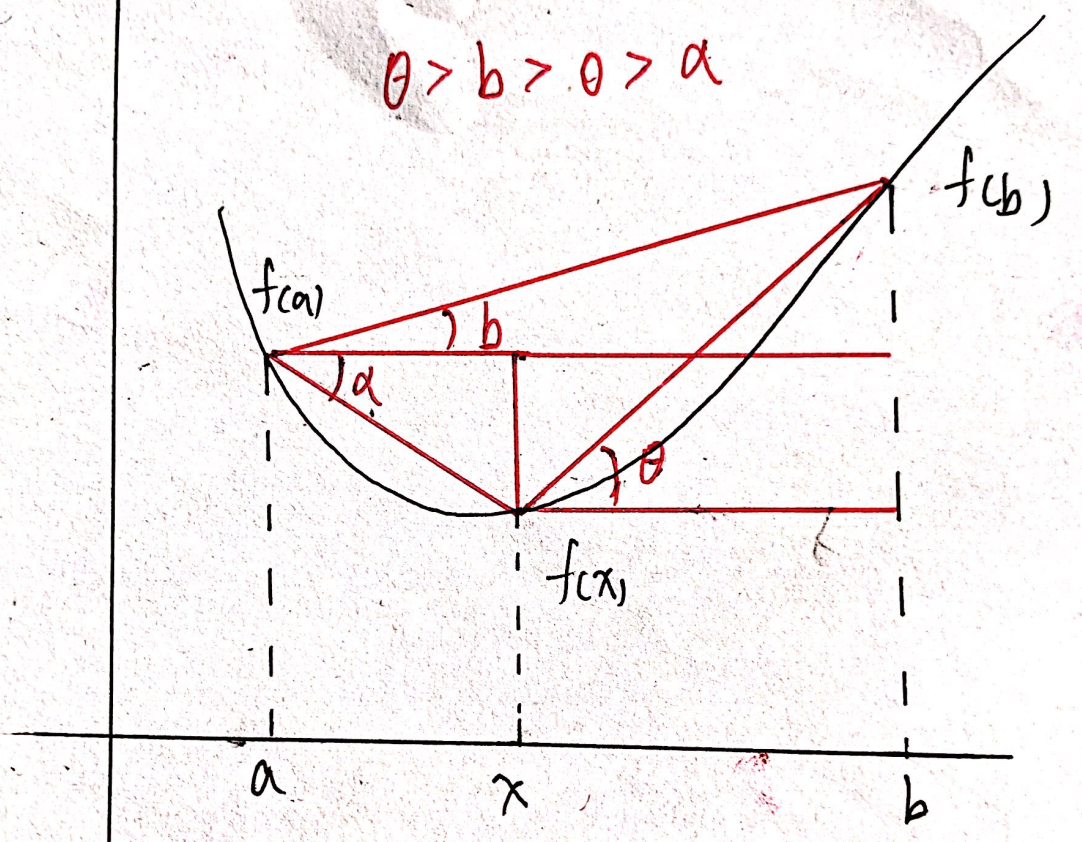
\includegraphics[scale=0.25]{P1.jpg}
    \end{figure}
    \item (c) In (b), we have shown that $f(a)'\leq \frac{f(x)-f(a)}{x-a}$ and $\frac{f(b)-f(x)}{b-x}\leq f(b)'$
    \\Therefore, $f(a)'\leq\frac{f(b)-f(a)}{b-a}\leq f(b)'$
    \item (d) According to (c), $\forall \bigtriangleup x>0, f(a)'\leq f(a+\bigtriangleup x)'$ 
    \\$f(a)''=\lim_{\bigtriangleup x\rightarrow 0}\frac{f(a+\bigtriangleup x)'-f(a)'}{\bigtriangleup x}\geq0$
    \\Therefore $f(a)''\geq0, f(b)''\geq0$
\end{enumerate}}}


\section*{Problem 2}\label{e-lin-frac-image}%
\emph{Composition with an affine function.}
Show that the following functions  $ f:\reals^n\rightarrow \reals $ are convex.
\begin{enumerate}
\item
 $ f(x) = \|Ax - b\| $ , where  $ A\in\reals^{m\times n} $, $ b\in\reals^m $, and  $ \|\cdot\| $  is a norm on  $ \reals^m $ .

\item
 $ f(x) = -\left( \det(A_0 + x_1 A_1 + \cdots + x_n A_n \right))^{1/m} $, on  $ \{x \;|\; A_0 + x_1 A_1 + \cdots + x_n A_n \succ 0\} $, where $ A_i \in \symm^m $.

\item
 $ f(X) = \Tr \left(A_0 + x_1A_1 + \cdots + x_n A_n \right)^{-1} $, on  $ \{x \;|\; A_0 + x_1 A_1 + \cdots + x_n A_n \succ 0 \} $, where $ A_i \in \symm^m $ .
(Use the fact that  $ \Tr (X^{-1})  $  is convex on $ \symm^m_{++} $ ; see exercise~3.18 in the text book.)
\end{enumerate}

{\bf{Answer:
\begin{enumerate}
    \item (a) According to definition, the norm must satisfy triangular inequality:
    \\$f(a+b)\leq f(a)+f(b)$
    \\Let $a=\theta x, b=(1-\theta)y$, we can get $f(\theta x+(1-\theta)y)\leq f(\theta x)+f((1-\theta)y)=\theta f(x)+(1-\theta)f(y)$
    \\So norm is a convex function
    \\It's clear that $g(x)=Ax-b$ is an affine function.
    \\Therefore $f(x)$, the composition of norm and an affine function, is convex.
    \item (b) Let $h(X)=-(\det X)^{1/m}$, by restricting it to a line we get $H(t)=h(X+tV)$
    \\$H(t)=-(\det(X+tV))^{1/m}=-(\det X)^{1/m}(\det(1+X^{-1/2}tVX^{-1/2}))^{1/m}$
    \\$H(t)=-(\det(X+tV))^{1/m}=-(\det X)^{1/m}(\prod_{i=1}^m(1+t\lambda_i))^{1/m}$ where $\lambda_i$ is the eigenvalue of $X^{-1/2}VX^{-1/2}$
    \\Then, both $H(t)$ and $h(X)$ are convex functions.
    \\\\Let $g(x)=A_0+x_1A_1+\cdots+x_nA_n$, then $g(x)\preceq 0, g(x)\in \dom f$
    \\Then $h(X)=-(\det X)^{1/m}$ is convex, and $g(x)$ is an affine transformation
    \\Therefore $f(x)$, the composition of a convex function and an affine function, is convex.
    \item (c) $\Tr(X^{-1})=\sum_{i=1}^m\frac{1}{\lambda_i}$, where $\lambda_i$ is the eigenvalue of $X$ 
    \\Then $Tr(X^{-1})$ is convex.
    \\Let $g(x)=A_0+x_1A_1+\cdots+x_nA_n$, then $g(x)\preceq 0, g(x)\in \dom f$
    \\Since $h(X)=\Tr (X)=X^{-1}$ is convex, and $g(x)$ is an affine transformation
    \\$f(x)$, the composition of a convex function and an affine function, is convex.
\end{enumerate}    
}}

\section*{Problem 3}\label{exe-sep-hyp-strict-counterexample}
\emph{Young's inequality. } Let  $ f:\reals\rightarrow \reals $  be an increasing function, with
$ f(0)=0 $ , and let  $ g $  be its inverse. Define  $ F $  and  $ G $  as
\[
F(x) = \int_0^x f(a) \,da, \qquad  G(y) = \int_0^y g(a) \,da.
\]
Show that  $ F $  and  $ G $  are conjugates, which then leads to the Young's inequality,
\[
xy \leqslant F(x) + G(y).
\]

{\bf{Answer:
\\Obviously, $F(x),G(y)$ is convex and increasing, with $F(0)=G(0)=0$.  
\\$F^*(y)=yx-F(x)$ where $y=F(x)'=f(x)$
\\Since $g(y)$ is the inverse function of $f(x)$, then $x=g(y)$
\\Therefore $F^*(y)=yg(y)-F(x)$ 
\\Since $F(x)=yg(y)-G(y)$
\\Then $F^*(y)=G(y)$, which means $F$ and $G$ are conjugates.
\\According to Fenchel inequality, $F(x)+G(y)\geq xy$
}}

%%%%%%%%%%%%%%%%%%%%%%%%%%%%%%%%%%%%%%%%%%%%%%%%%%%%%%%%%%%%%%%%%%%%
% Reference
%%%%%%%%%%%%%%%%%%%%%%%%%%%%%%%%%%%%%%%%%%%%%%%%%%%%%%%%%%%%%%%%%%%%
\end{document}
